%/sw/bin/dvips -Ppdf -G0 isba14.poster
% check that dvips is not aliased with -t letter
\documentclass[a0,landscape]{a0poster}
\usepackage{graphicx,amsmath,amssymb,color}
\usepackage[absolute,overlay]{textpos}
\usepackage{natbib}
\usepackage{wrapfig}

\definecolor{bgcolor}{rgb}{.89,1,.78}
\definecolor{bgcolor2}{rgb}{.8,1,1}
\definecolor{bgcolor3}{rgb}{.9,.9,1}
\definecolor{EmphCol}{rgb}{0,0,.45}
\definecolor{EmphCol2}{rgb}{.35,0,0}

\newcommand{\boldgreek}[1]{\mbox{\boldmath $#1$}}

\TPGrid[20mm,20mm]{25}{15}  % 3 - 1 - 7 - 1 - 3 Columns
\textblockcolor{}
%\TPMargin{5mm}

\definecolor{blue}{rgb}{0.000,0.000,1.000}         %Blue1
\definecolor{darkaqua}{rgb}{0.000,0.749,1.000}     %DeepSkyBlue1
\definecolor{magenta}{rgb}{1.000,0.000,1.000}      %magenta1
\definecolor{green}{rgb}{0.396,0.864,0.396}        %LimeGreen
\definecolor{brown}{rgb}{0.722,0.525,0.043}        %DarkGoldenrod     
\definecolor{purple}{rgb}{0.706,0.322,0.804}       %MediumOrchid2
\definecolor{red}{rgb}{1.000,0.000,0.000}          %red
\newcommand{\co}[2]{{{\bf \color{#1}{#2}}}}

\begin{document}

%% title and authors 
\begin{textblock}{25}(0,0)

\begin{center}
\vspace{1cm}
{\veryHuge  \textsf{Determining Convergence in Gaussian Process Surrogate Model Optimization}}\\
\vspace{1cm}
\noindent{\Large \textsf{{\LARGE Nicholas Grunloh} and {\LARGE Herbie Lee} (Applied Mathematics and
    Statistics, Baskin School of Engineering, University of
    California, Santa Cruz)}}\\
\vspace{1cm}
\end{center}

\end{textblock}

%\begin{textblock}{.5}(1,0)
%\includegraphics[scale=2.75]{slug}
%\end{textblock}
%
%\begin{textblock}{.5}(20.8,0.2)
%\includegraphics[scale=1.8]{SOE_logo}
%\end{textblock}

%column 1
\begin{textblock}{6}(1,1.3)
%\textblockcolour{bgcolor3}
\begin{center}
{\LARGE \textsc{\co{darkaqua}{Abstract}}}\\
\end{center}
\medskip

\large
\noindent 
Identifying convergence in numerical optimization is an ever-present, difficult, and often subjective task. 
The statistical framework of Gaussian process surrogate model optimization provides useful measures for tracking optimization progress; however, the identification of convergence via these criteria has often provided only limited success and often requires a more subjective analysis. 
Here we develop a novel approach that adapts ideas originally introduced in the field of statistical process control to define a robust convergence criterion based upon the improvement function. 
\end{textblock}

\begin{textblock}{6}(1,4.05)
%\textblockcolour{bgcolor}

\begin{center}
\LARGE \textsc{\co{green}{Gaussian Process Surrogates}}\\
\end{center}
\medskip

\large
\noindent
The typical approach to modeling a black-box function is with a
Gaussian Process (GP) surrogate model \citep{santnerBook}:
\[ Y(\mathbf{x}) = \boldgreek{\beta}'\mathbf{h}(\mathbf{x}) +
Z(\mathbf{x}) + \epsilon \]
where $Y$ is a scalar output, $\boldgreek{\beta}$ is a vector of
regression coefficients, $h$ is typically the identity function plus
inclusion of an intercept, and $Z$ a zero-mean GP with spatial
covariance kernel $C(\cdot,\cdot)$ and possible error term (nugget)
$\epsilon\sim N(0,\sigma_{\epsilon}^2)$. Following the literature, we
use a Gaussian correlation structure $K(\mathbf{x}_i,\mathbf{x}_j) =
\exp\left\{- \sum_{k=1}^m (x_{ik}-x_{jk})^2/d_k\right\}$.
For additional flexibility, we used Treed Gaussian Processes
\citep{gramacy2012}, which allows for non-stationarity and possible
discontinuities.
\end{textblock}

\begin{textblock}{6}(1,7.7)

\begin{center}
\LARGE \textsc{\co{blue}{Optimization with Expected Improvement}}\\
\end{center}
\large

\noindent
Global minimization can be attempted using a surrogate model by
sequentially choosing a new function evaluation at the input that
maximizes the expected improvement (EI), where the improvement
function is 
\[ I(\mathbf{x}) = \max\left\{ y_{min}-Y(\mathbf{x})\;,\; 0\right\} \]
where $y_{min}=\min\{y_1,\ldots,y_n\}$ and the expectation is taken
with respect to the posterior predictive distribution of the
surrogate \citep{jonesEIOpt}. We can do optimization by sequentially
evaluating the point with the largest EI at each iteration, then
updating the model and repeating. But when do you stop?

\end{textblock}

\begin{textblock}{6}(1,11.1)

\begin{center}
\LARGE \textsc{\co{purple}{When to Declare Convergence?}}\\
\end{center}
\large

\noindent
Some have suggested using EI for convergence \citep{windExample}, 
declaring convergence when the largest EI value falls below a pre-determined
threshold, much like many stopping criteria in numerical algorithms.
The idea is that our surrogate model predicts that there is very low 
probability of finding any other points that are more optimal.

\vspace{0.3in}
\noindent
However, this approach ignores the fact that EI is a random variable
and oversimplies the stochastic nature of convergence in this setting.
Thus it results in inconsistent behavior.
\end{textblock}

% column 2

%\begin{textblock}{4.3}(10.04,2)
%\textblockcolour{bgcolor2}
%\begin{center}
%{\LARGE \textsc{Example Data Plots}}\\
%\end{center}
%\end{textblock}

\begin{textblock}{7.8}(7.3,1.3)

\begin{center}
\LARGE \textsc{\co{red}{Examples of EI Monitoring}}\\
\end{center}
\large

\noindent
Three examples of Expected Log-normal Approximation to the Improvement (ELAI),
where the log scale is used because EI is strictly positive but decreasingly
small:

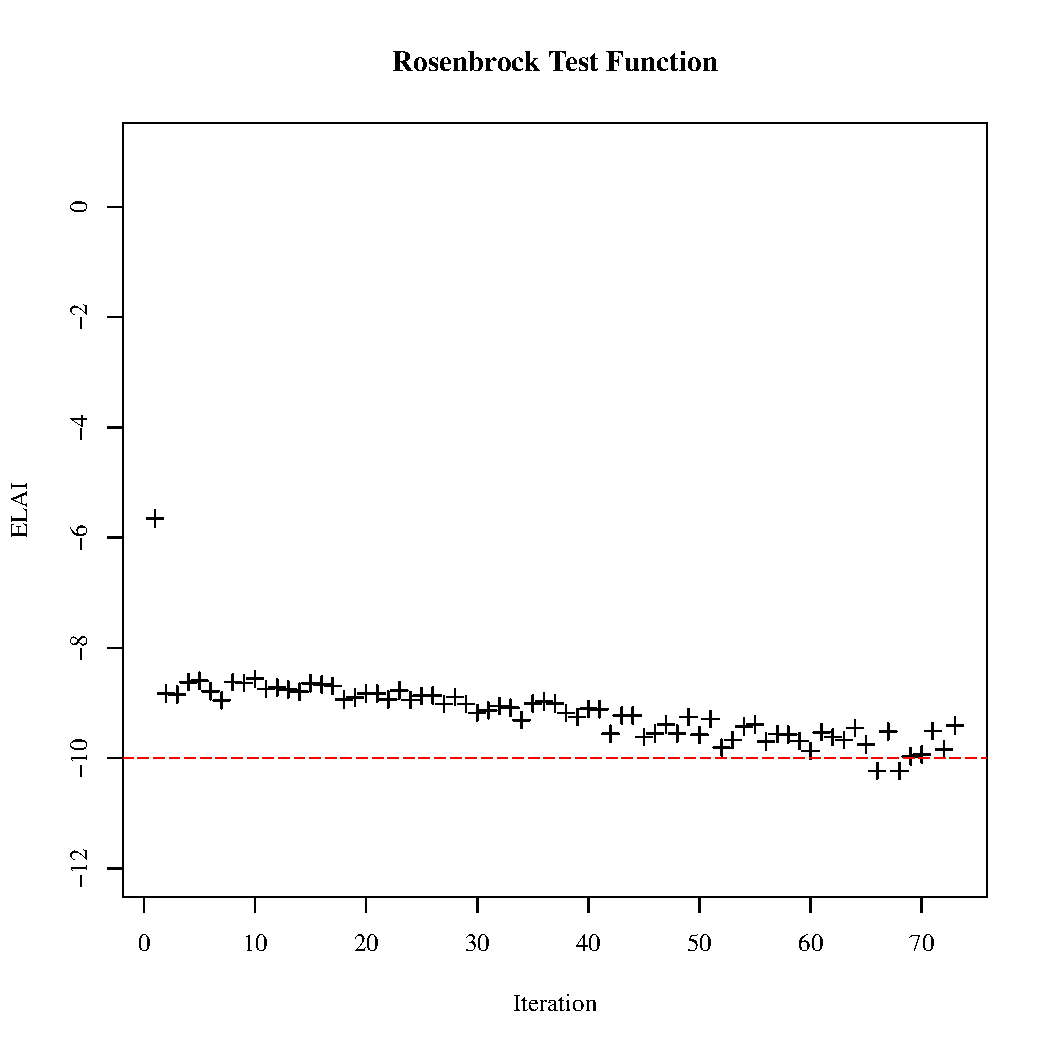
\includegraphics[width=0.33\textwidth]{./figures/introChartRoseEasyEasyAxis.pdf}
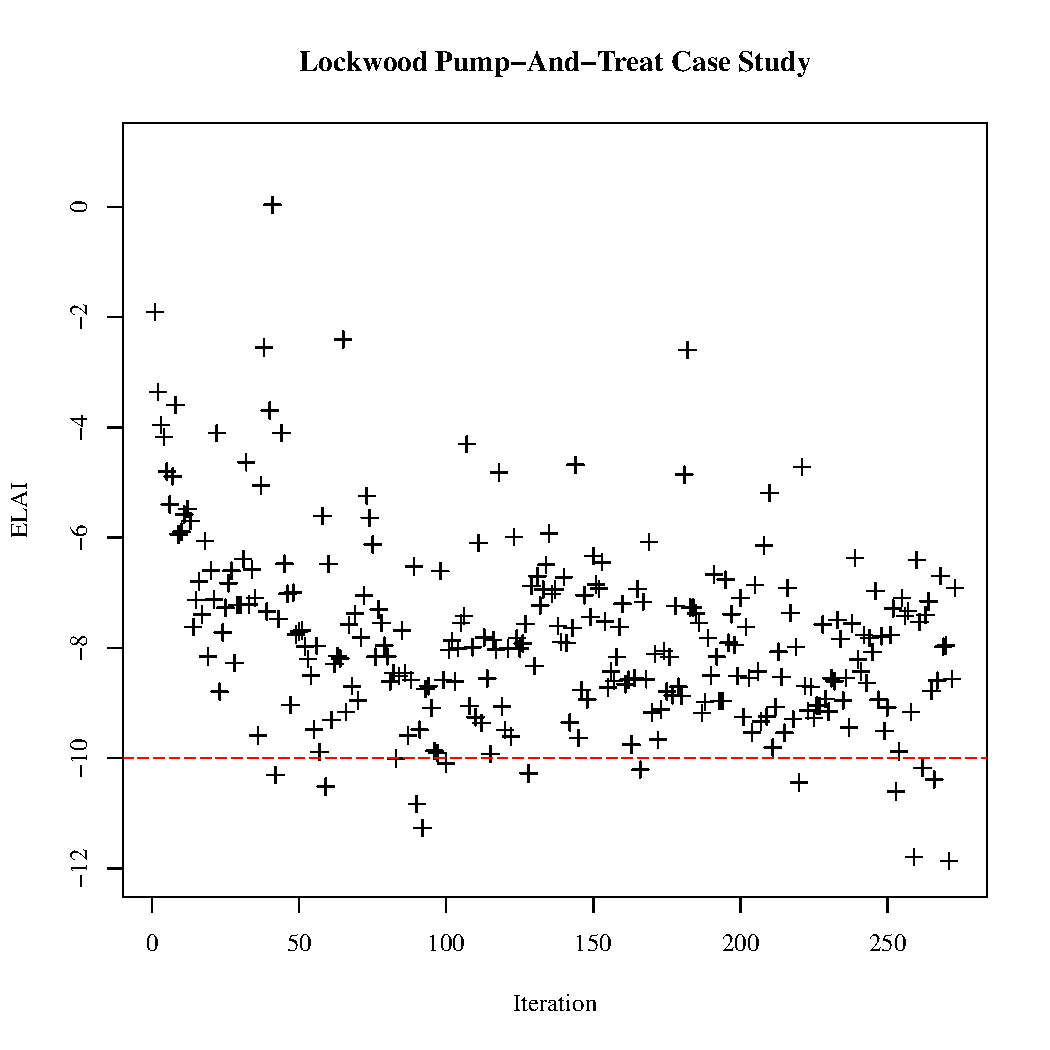
\includegraphics[width=0.33\textwidth]{./figures/introChartLock6Three20000Axis.pdf}
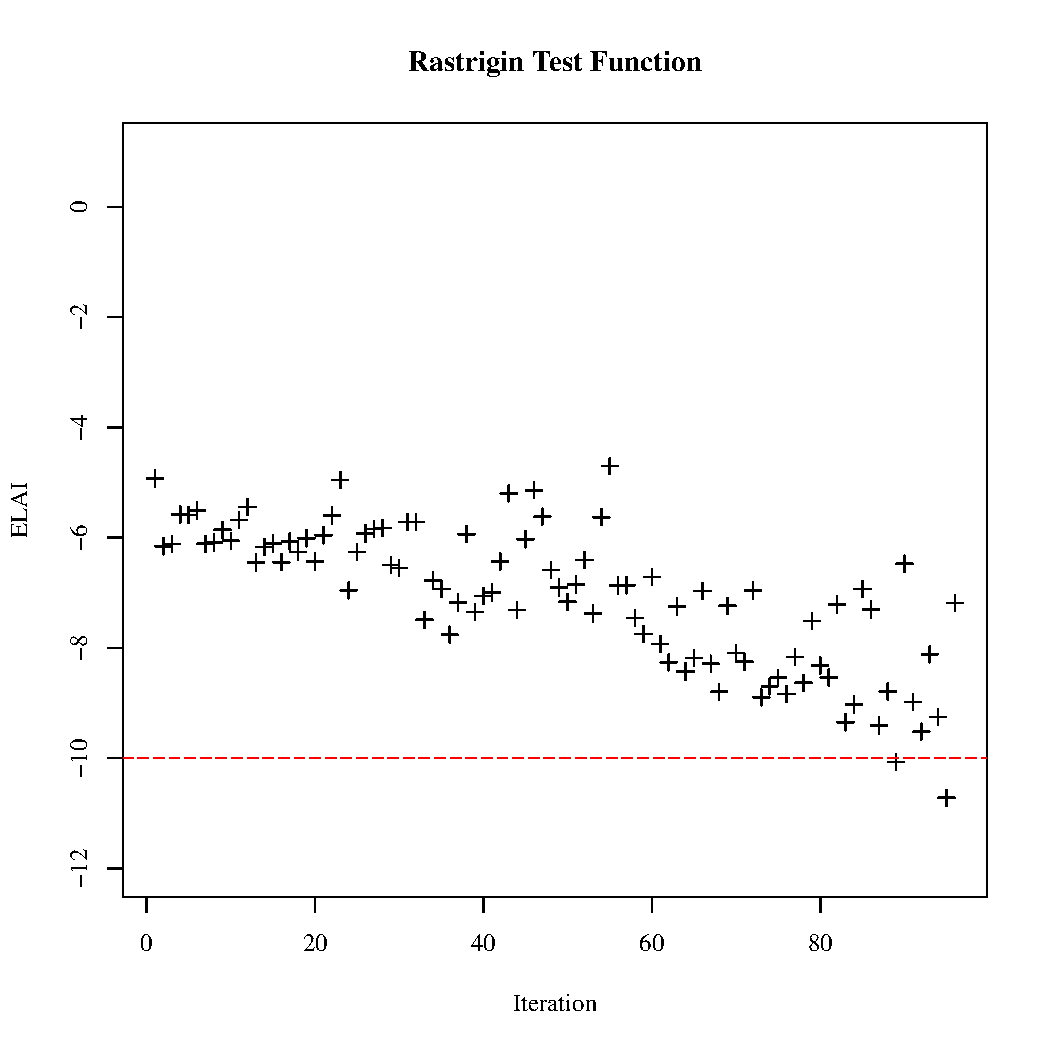
\includegraphics[width=0.33\textwidth]{./figures/introChartRastHardAxis.pdf}


\noindent
The first example (Rosenbrock) is an ideal well-behaved case, where convergence
does occur when the threshold is met. The second example (Lockwood) shows a
failure of the threshold, as it is met too early, and while the
variability is still too large. But small variability is also not sufficient
or necessary, as the third example shows, where variability is increasing but 
meeting the threshold does indicate convergence.

\vspace{0.3in}
\noindent
Working on the log sacle is important because the EI distribution is right
skewed, and become more skewed as convergence approaches. Numerically, some
EI values get evaluated to be 0 in double precision, even though they
are theoretically positive. Thus we use a model-based approximation of a
log-normal, transforming the empirical mean and variance via the log-normal.
\end{textblock}

\begin{textblock}{7.8}(7.3,7.1)
\begin{center}
\LARGE \textsc{\co{brown}{Statistical Process Control}}\\
\end{center}
\large

\noindent
Consider a control chart, used to monitor a process in equilibrium to watch
for it to deviate (go out of control). We take inspiration from this approach,
but use it in reverse. As optimization proceeds, EI decreases as
we find lower values and learn more about the function. Once we find the
minimum, we achieve convergence, and at this point, EI should
settle into an approximately stable distribution. Thus we want to see when our
out of control process becomes an in-control process.

\vspace{0.3in}
\noindent
We basically perform SPC backwards in time. Starting with the most recent
iteration, we look backwards in time and see if we have an in-control process that
becomes out of control. That is the signature of convergence. 

\vspace{0.3in}
\noindent
We use an Exponentially Weighted Moving Average (EWMA) control chart
\citep{ewmaPaper}, which provides smoothing to account for highly
stochastic nature of EI. The exponential weighting also helps when the 
series is decreasing, as is typical pre-convergence. Denote the ELAI
values by $Y_i$. EWMA tracks $Z_i = \lambda Y_i + (1-\lambda)Z_{i-1}$. 
\end{textblock}

\begin{textblock}{7.8}(7.3,11.2)
\begin{center}
\LARGE \textsc{\co{green}{Control Window}}\\
\end{center}
\large

\noindent
We define a control window of the $w$ most recent observations from which we 
compte the control limits of the EWMA chart. Starting from the most recent
point in time, we look backwards, using the first $w$ observations to get
the control limits, then looking to see if any points further back in time
go outside those limits. If so, we declare convergence. If we are 
pre-convergence, then the $w$ points won't be in equilibrium and the
control limits will be quite large, typically including all runs from
the beginning.

\vspace{0.3in}
\noindent
The choice of $w$ depends on the difficulty of the problem, it needing
to be sufficiently large to establish control, but not too large as
that means extra iterations beyond those necessary. 
Our default is $w=15p$ where $p$ is the dimension of the problem.
\end{textblock}

%% column 3

%\begin{textblock}{6.7}(16.84,2)
%\textblockcolour{bgcolor2}
%\begin{center}
%{\LARGE \textsc{Example Representative Point Plots}}\\
%\end{center}
%\end{textblock}

\begin{textblock}{8.8}(15.3,1.3)
\begin{wrapfigure}{r}{0.73\textwidth}
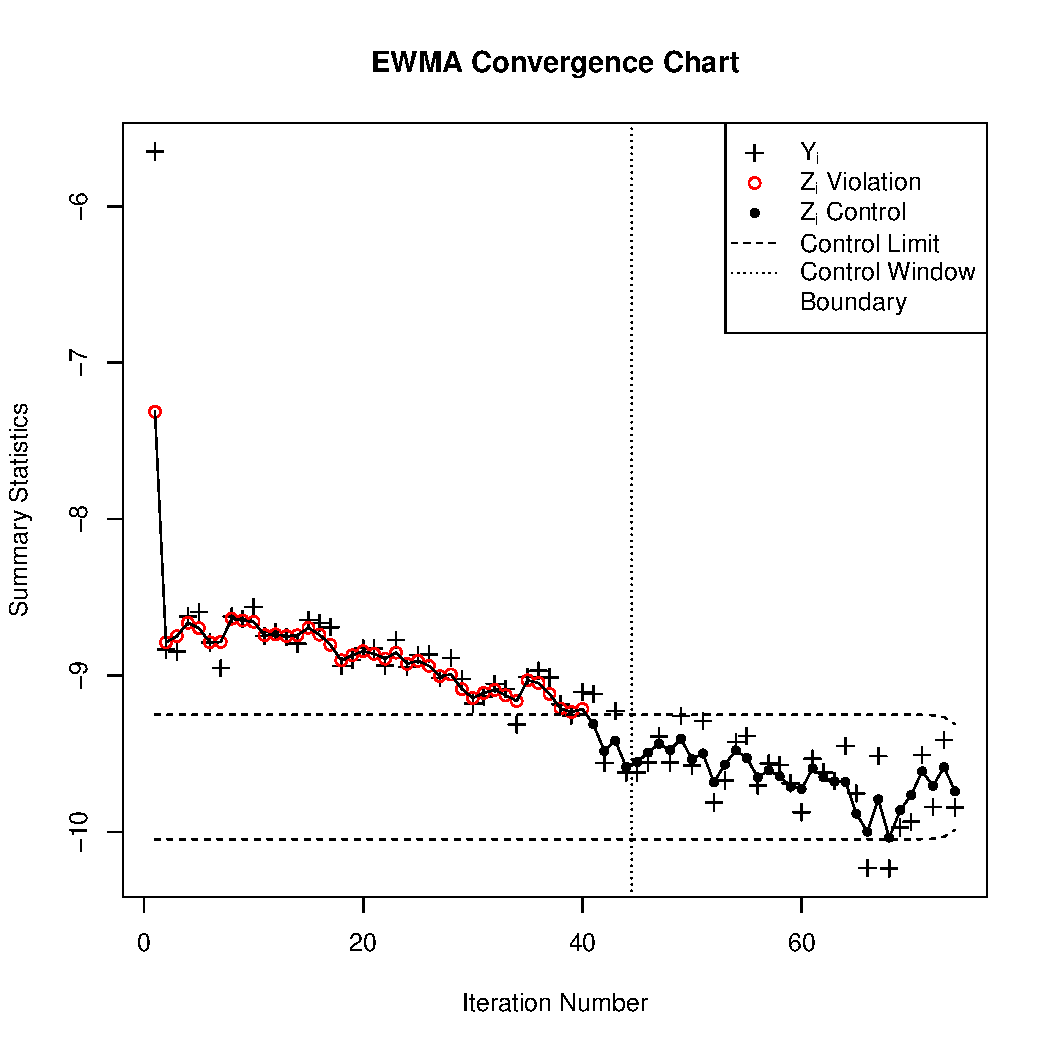
\includegraphics[width=0.35\textwidth]{./figures/ewmaConvChartRoseEasyEasyBW.pdf}
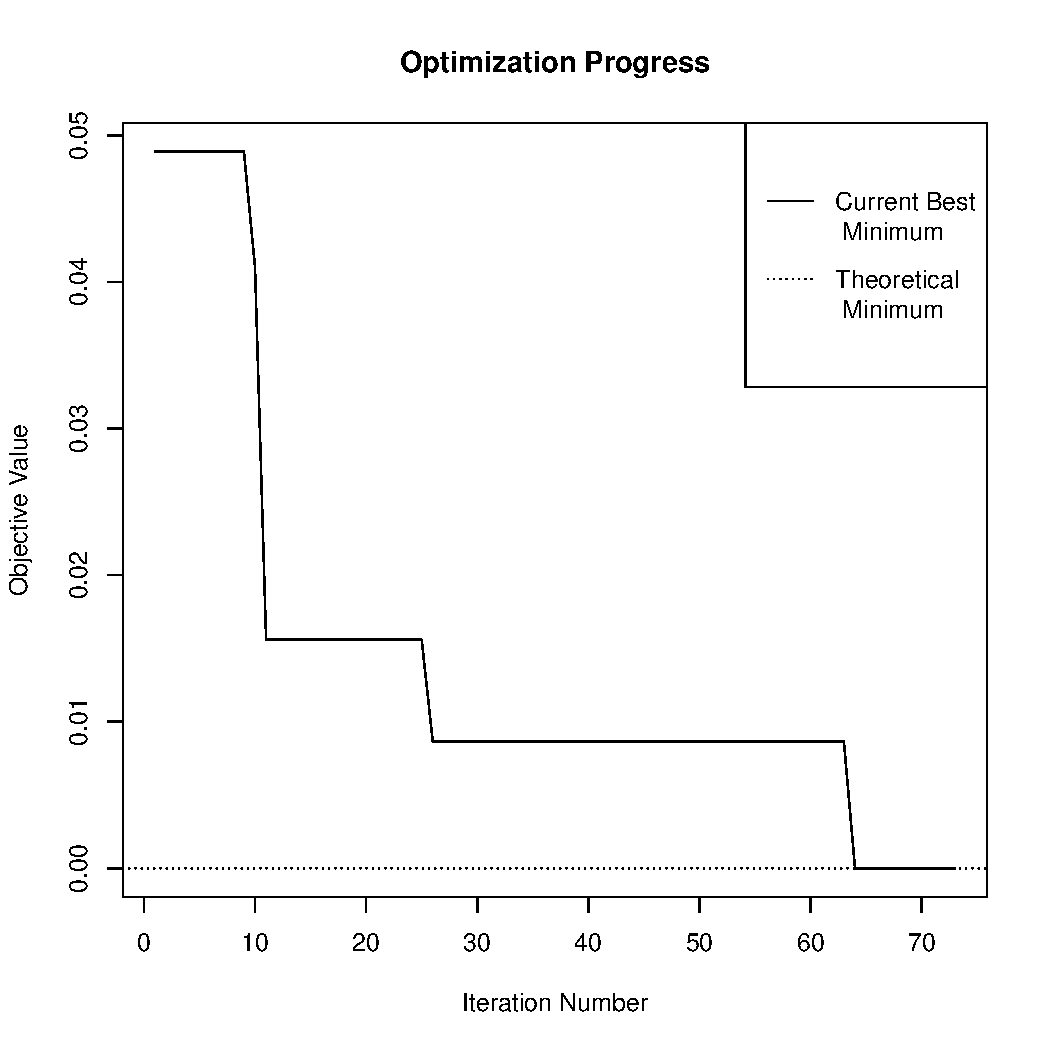
\includegraphics[width=0.35\textwidth]{./figures/bestZRoseEasyEasyEnd.pdf}
\end{wrapfigure}

\vspace*{0.05in}
\noindent
\textsc{\LARGE\co{blue}{Rosenbrock}}

\vspace{0.06in}
\noindent
\textsc{\LARGE\co{blue}{Test Function}}

\large
\noindent
$f(x_1, x_2) =$\\ 
$100\left(x_2 \!-\! x_1^2\right)^2 \!+\! (1\!-\! x_1)^2$.\\
We use $w=30$ and estimate $\hat\lambda\approx 0.5$. The EWMA convergence
chart goes into control as we find the true global minimum.
\end{textblock}

\begin{textblock}{8.8}(15.3,4.3)
\begin{wrapfigure}{r}{0.73\textwidth}
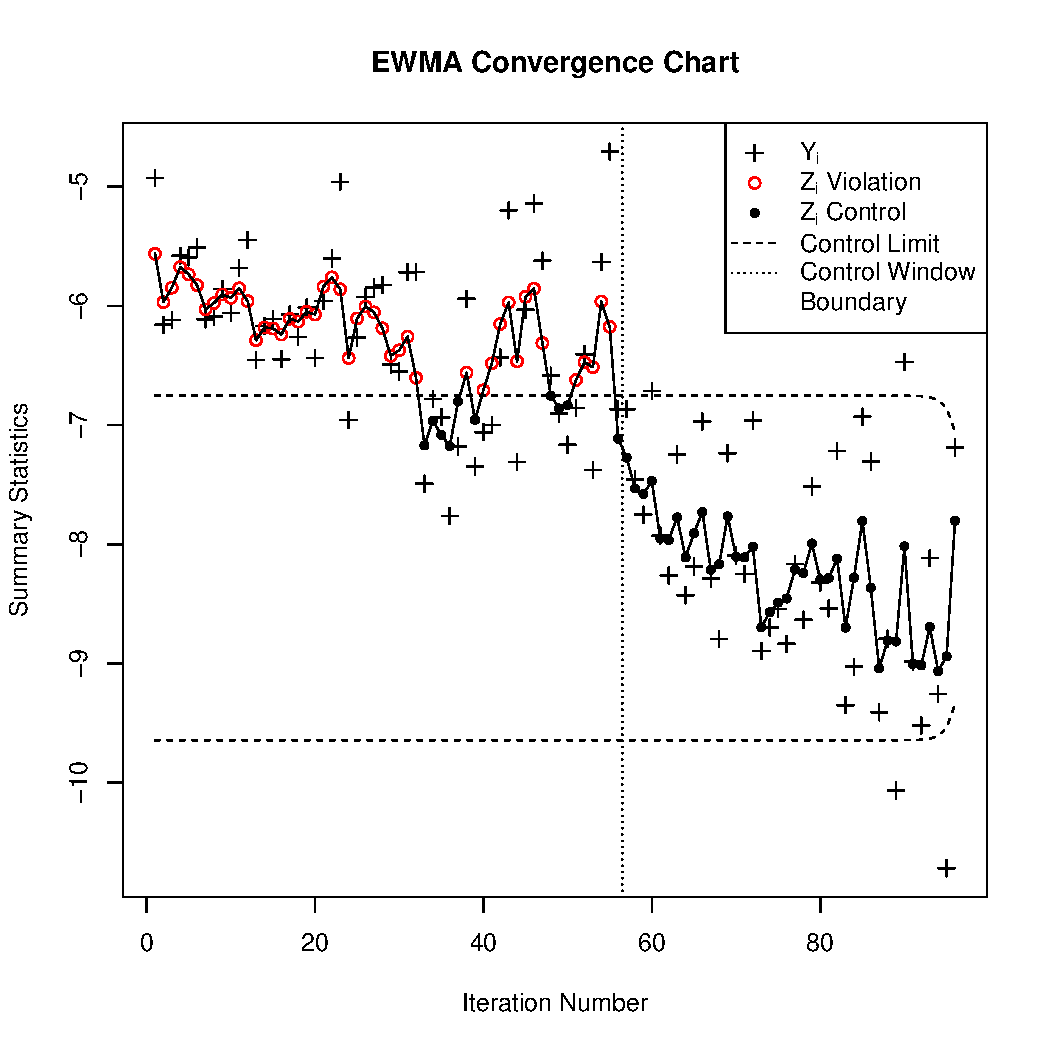
\includegraphics[width=0.35\textwidth]{./figures/ewmaConvChartRastHardBW.pdf}
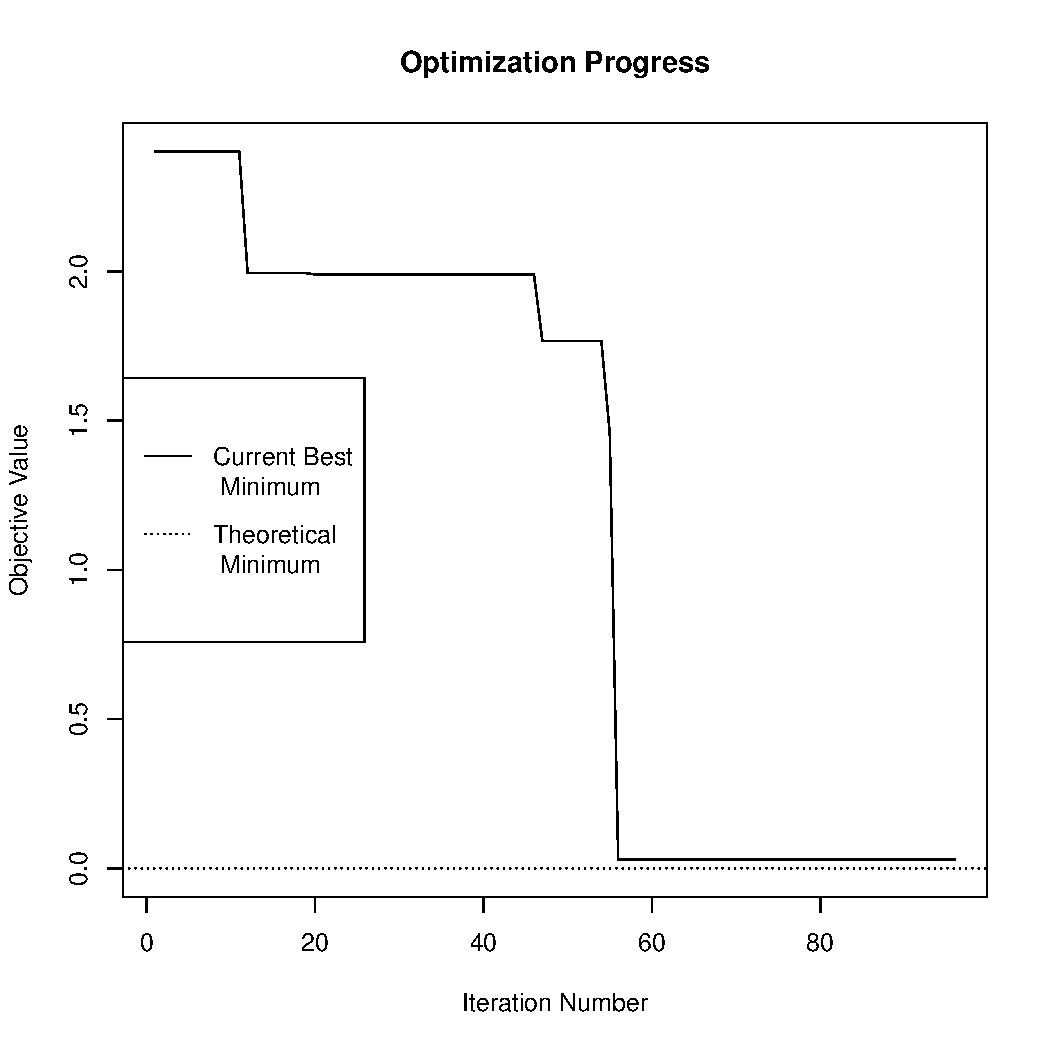
\includegraphics[width=0.35\textwidth]{./figures/bestZRastHardEnd.pdf}
\end{wrapfigure}

\vspace*{0.05in}
\noindent
\textsc{\co{blue}{\LARGE Rastrigin}}

\vspace{0.06in}
\noindent
\textsc{\co{blue}{\LARGE Test Function}}
\large

\noindent
This highly multi-modal function is $f(x_1, x_2) =
\sum_{i=1}^2\left[x_i^2-10\cos(2\pi x_i)\right] + 2(10)$.  
We use $w=40$ and estimate $\hat\lambda\approx 0.4$. It takes a little
time after finding the global minimum for the EWMA convergence
chart to establish convergence.
\end{textblock}

\begin{textblock}{8.8}(15.3,7.5)
\begin{wrapfigure}{r}{0.73\textwidth}
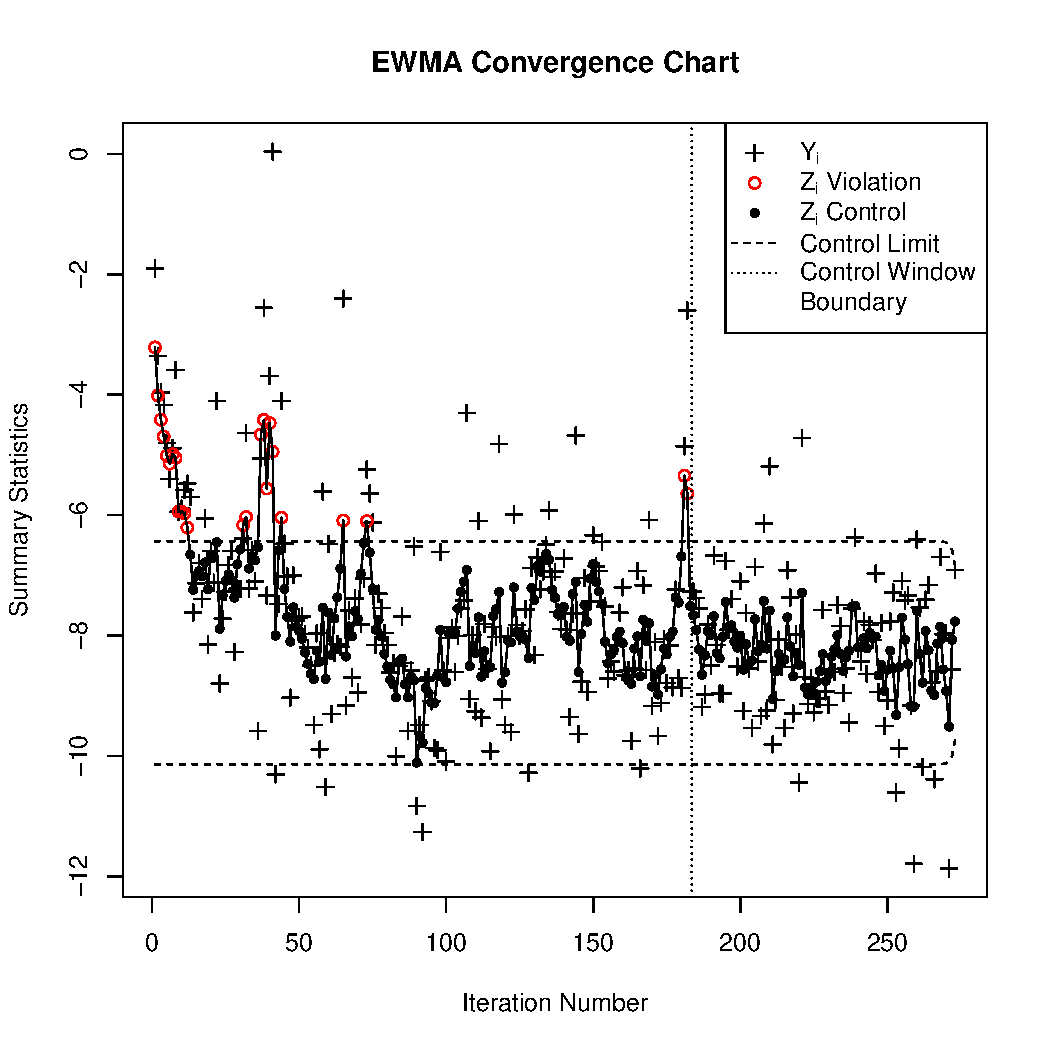
\includegraphics[width=0.35\textwidth]{./figures/ewmaConvChartLock6Three20000End.pdf}
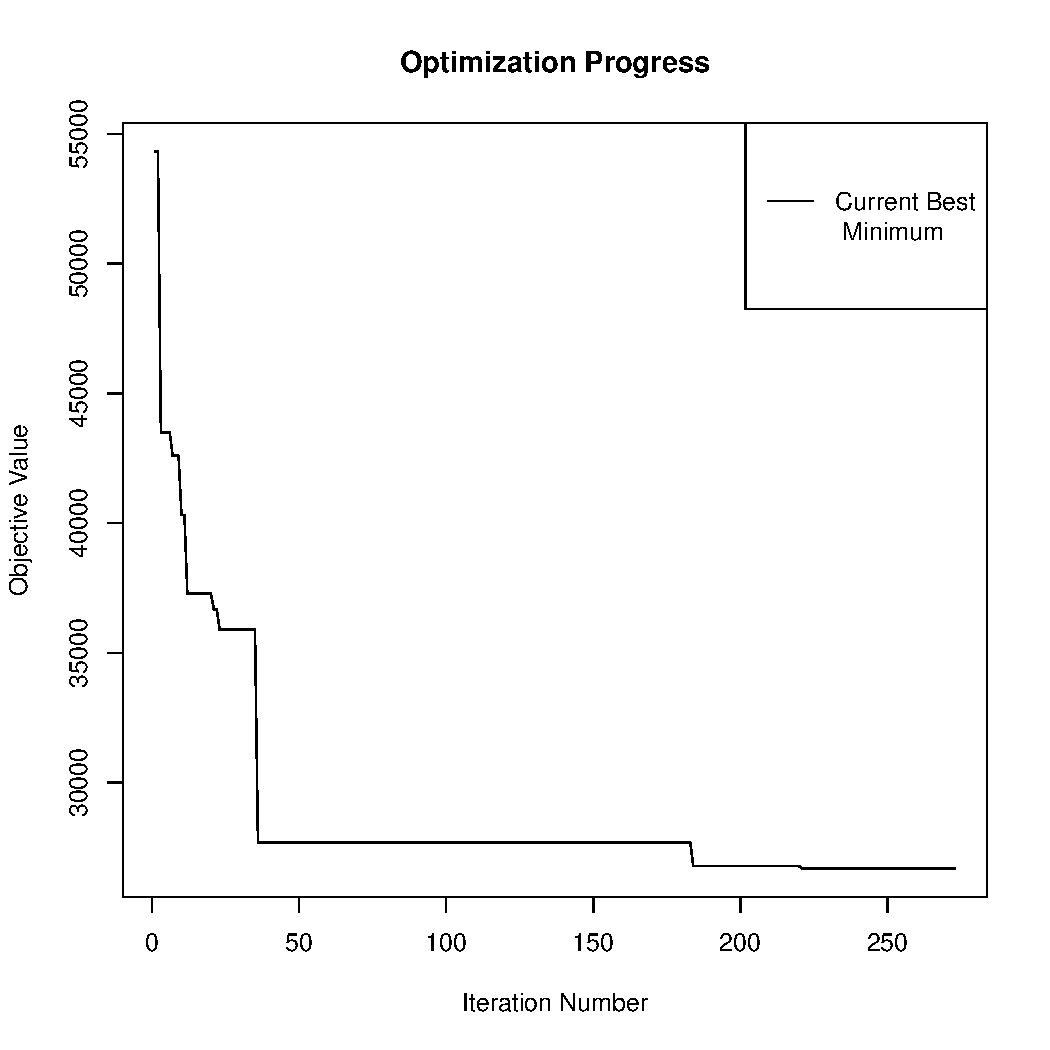
\includegraphics[width=0.35\textwidth]{./figures/bestZLock6Three20000End.pdf}
\end{wrapfigure}

\vspace*{0.05in}
\noindent
\textsc{\co{blue}{\LARGE Lockwood}}

\vspace*{0.06in}
\noindent
\textsc{\co{blue}{\LARGE Case Study}}

\large

\noindent
For this six-dimensional groundwater remediation problem from
\citet{mayer2002optimal}, the objective is 
to find the lowest operation cost configuration
(pumping rates) of six extraction wells while avoiding  
spread of the contamination. 
We use $w=90$ and estimate $\hat\lambda\approx 0.4$.
\end{textblock}

\begin{textblock}{8.8}(15.3,10.85)

\bibliographystyle{jasa}
\bibliography{spcCite}

\end{textblock}


\end{document}





